\clearpage
\phantomsection

\setcounter{chapter}{3}
\chapter[{MÔ PHỎNG VÀ KIỂM THỬ}]{mô phỏng và kiểm thử}
Để đánh giá độ chính xác của thiết kế, một bước quan trong trong quá trình thiết kế là cần có các bài mô phỏng và các trường hợp kiểm thử. Chương 4 sẽ mô tả chi tiết về một số phương pháp kiểm thử được sử dụng, các điều kiện để đánh giá độ chính xác của kiểm thử, mô hình giúp tự động hóa quá trình kiểm thử.
\section{Cơ sở lý thuyết kiểm thử}
\subsection{Lý thuyết về độ bao phủ}
Độ bao phủ (coverage) là phương pháp thống kê trong quá trình kiểm tra thiết kế để xác định được chất lương của quá trình kiểm tra. Độ bao phủ là một yếu tố quan trọng để khẳng định được thiết kế có được kiểm tra theo các yêu cầu đưa ra hay chưa. Từ đó, có thể xem xét tạo ra các bài kiểm tra để đảm bảo bao quát được các trường hợp.

Có hai yếu tố bao phủ thường được đánh giá là độ bao phủ về mã nguồn (code coverage) và độ bao phủ về mặt chức năng (functional coverage). Trong đó, độ bao phủ về mã nguồn sẽ đánh giá xem là các điều kiện ví dụ các điều kiện rẽ nhánh có được thực hiện ít nhất 1 lần hay không, do đó nó không có ý nghĩa về mặt đánh giá độ chính xác của thiết kế mà chỉ đảm bảo rằng bộ kiểm thử sinh ra đã bao quá được hết mã nguồn. Độ bao phủ về mặt chức năng sẽ đánh giá độ bao phủ của thiết kế dựa trên tính năng đã được kiểm tra. Do đó, việc định nghĩa ra các tính năng nào cần được đánh giá sẽ quyết định chất lượng của độ bao phủ về mặt chức năng. Độ bao phủ về mặt mã nguồn thường được thu thập từ các phần mềm sử dụng để thiết kế ví dụ Vivado, QuetaSim,... Trong khi đó, độ bao phủ về mặt chức năng phải do kỹ sư tự định nghĩa, kỹ sư cần tự định nghĩa điểm cần bao phủ. Ví dụ về kiểm tra về mặt chức năng, giả sử kỹ sư cần kiểm tra một biến có thay đổi theo như mong muốn hay không. Nếu đúng, biến đấy phải thay đổi giá trị từ 3 -> 5 -> 7 chẳng hạn. Độ bao phủ về mặt mã nguồn chỉ biết là biến đấy đã thành 3, 5 hoặc 7 mà không thể đánh giá được về mặt thứ tự xuất hiện.

\subsection{Các phương pháp kiểm thử}
Trong thiết kế nói chung, sau khi đã thiết kế được các mạch từ mã nguồn hoặc thông qua các công cụ, kỹ sư cần thiết kế các bài kiểm thử để đánh giá tính đúng đắn của thiết kế. Thông thường, đối với thiết kế số, kỹ sư sẽ thiết kế ra các phương pháp kiểm thử trực tiếp (directed testing). Khi sử dụng phương pháp này, kỹ sư sẽ nhìn vào các yêu cầu kỹ thuật, viết ra các trường hợp có thể xảy ra và kiểm tra nó với một kết quả đã biết trước. Để kiểm tra, kỹ sư có thể nhìn dạng sóng mô phỏng, sử dụng các điều kiện để kiểm tra. Đây là một phương pháp nhanh, phù hợp với kỹ sư cần kiểm tra ngay lập tức thiết kế là đúng hay sai, nhưng sẽ khó để đảm bảo hoàn toàn về mặt thiết kế. Giả sử, nếu thiết kế có 10, 100 tín hiệu đầu vào, vậy nếu viết tay và tính toán các trường hợp kiểm thử sẽ rất tốn thời gian và có thể dễ mắc đến các sai lầm.

Vậy để có thể kiểm tra được toàn bộ thiết kế một cách đầy đủ, các kỹ sư sẽ thiết kế ra các kích thích sinh ngẫu nhiên với ràng buộc (constrained-random stimulus). Các kích thích này sẽ sinh ra các tín hiệu ngẫu nhiên giá trị, tuy nhiên phải tuân theo các ràng buộc cho trước. Ví dụ, kỹ sư có thể yêu cầu khi sinh ra dữ liệu điểm ảnh, thì tín hiệu hợp lệ phải ở mức 1. Từ đó, kỹ sư có thể kiểm tra được nhiều trường hợp hơn với những dữ liệu ngẫu nhiên đó. Hình \ref{fig:verificationEva} mô tả biểu đồ phân tích thời gian và độ bao phủ của các bộ kiểm thử. Có thể thấy, với cách tạo ra các kích thích trực tiếp, thời gian để đạt độ bao phủ cần thiết là rất lớn, trong khi đó với các kích thích được sinh ngẫu nhiên với các ràng buộc, thời gian này đã giảm đi một cách đáng kể.

\begin{figure}[!ht]
\centering
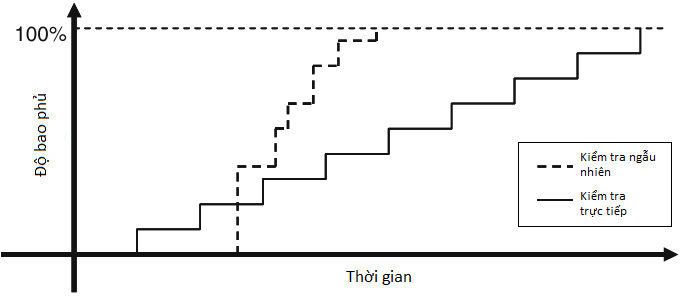
\includegraphics[width=\linewidth]{figures/verificationEva.png}
\caption{Biểu đồ phân tích thời gian và độ bao phủ của các bộ kiểm thử}
\label{fig:verificationEva}
\end{figure}

\section{Phương pháp xây dựng kiểm thử và kết quả}
Hình \ref{fig:testComponents} mô tả các thành phần cơ bản của một bộ kiểm tra, bao gồm testbench sẽ sinh ra các kích thích đầu vào và sau đó thu thập các dữ liệu đầu ra.
Trong khi thiết kế, kỹ sư sẽ cần kiểm tra ngay lập tức chức năng của một hoặc nhiều mô-đun để đảm bảo tính chính xác một cách chưa đầy đủ, tức là kiểm tra mô-đun đó đã hoạt động đúng tính năng mong muốn hay chưa, tuy nhiên có thể có những trường hợp ngoại lệ mà kỹ sư có thể không nghĩ đến. Do đó, thường thì kỹ sư sẽ kiểm tra bằng cách tạo ra các bộ kiểm thử với kích thích sinh trực tiếp để tiết kiệm về mặt thời gian. Do đó, đối với các mô-đun nhỏ, sinh viên sẽ tự đưa ra các bộ kích thích trực tiếp và sau đó kiểm tra kết quả với đầu ra đã có trước. 

\begin{figure}[!ht]
	\centering
	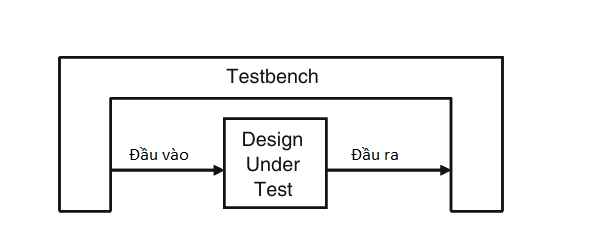
\includegraphics[width=\linewidth]{figures/testComponents.png}
	\caption{Các thành phần cơ bản của một bộ kiểm tra}
	\label{fig:testComponents}
\end{figure}

Tuy nhiên, để kiểm tra tự động với những đầu vào ngẫu nhiên đồng thời đánh giá về độ bao phủ của bộ kiểm tra, sinh viên đã định nghĩa ra một bộ kiểm thử có kiến trúc được mô tả tại hình \ref{fig:myLayeredtb}. \textit{Lưu ý: Ngôn ngữ sử dụng để xây dựng bộ kiểm tra phân tầng là SystemVerilog}. Về cơ bản, bộ kiểm tra này sẽ gồm các lớp thực hiện các chức năng riêng biệt theo một kịch bản đã định nghĩa trước. Đầu tiên là lớp Transaction, lớp này sẽ định nghĩa ra các giao dịch, các ràng buộc để tạo dữ liệu đầu và đồng thời đưa ra các phương thức để sao chép. Lớp Generator sẽ có nhiệm vụ thực hiện việc sinh ra các dữ liệu đầu vào và sau khi sinh xong hết, nó sẽ có một lời gọi hệ thống để chạy 1 bộ tính toán ra dữ liệu mong muốn ở bên ngoài bộ kiểm tra. Dữ liệu được sinh ra sẽ được đẩy xuống lớp Driver qua một cách vận chuyển gọi là mailbox. Đây là các để chuyển dữ liệu qua 2 lớp của ngôn ngữ SystemVerilog. Lớp Driver sẽ thực hiện hai phương thức chính là \textbf{reset} và \textbf{run}. Trong đó reset giúp khởi động lại toàn bộ hệ thống, còn run sẽ thực hiện đưa dữ liệu đó vào DUT để thực hiện tính toán. Lớp Monitor sẽ liên tục giám sát DUT, nếu đã có dữ liệu đầu ra, lớp này sẽ bắt lại nó, sau đó đưa vào lớp Scoreboard. Lớp Scoreboard sẽ đọc dữ liệu mong muốn và dữ liệu thực tế, so sánh và đưa ra đánh giá. Trong lúc tất cả các lớp khác đang hoạt động, lớp đánh giá độ bao phủ về mặt chức năng cũng đồng thời đánh giá các trường hợp. Sau khi đã kiểm tra hết số lượng kiểm thử đã định nghĩa, một báo cáo về độ bao phủ về mặt chức năng sẽ được đưa ra. Các event là một kiểu dữ liệu của SystemVerilog dùng để chờ hoặc kích hoạt nhằm đảm bảo kịch bản sẽ hoạt động chính xác theo trình tự. 
\begin{figure}[!hb]
	\centering
	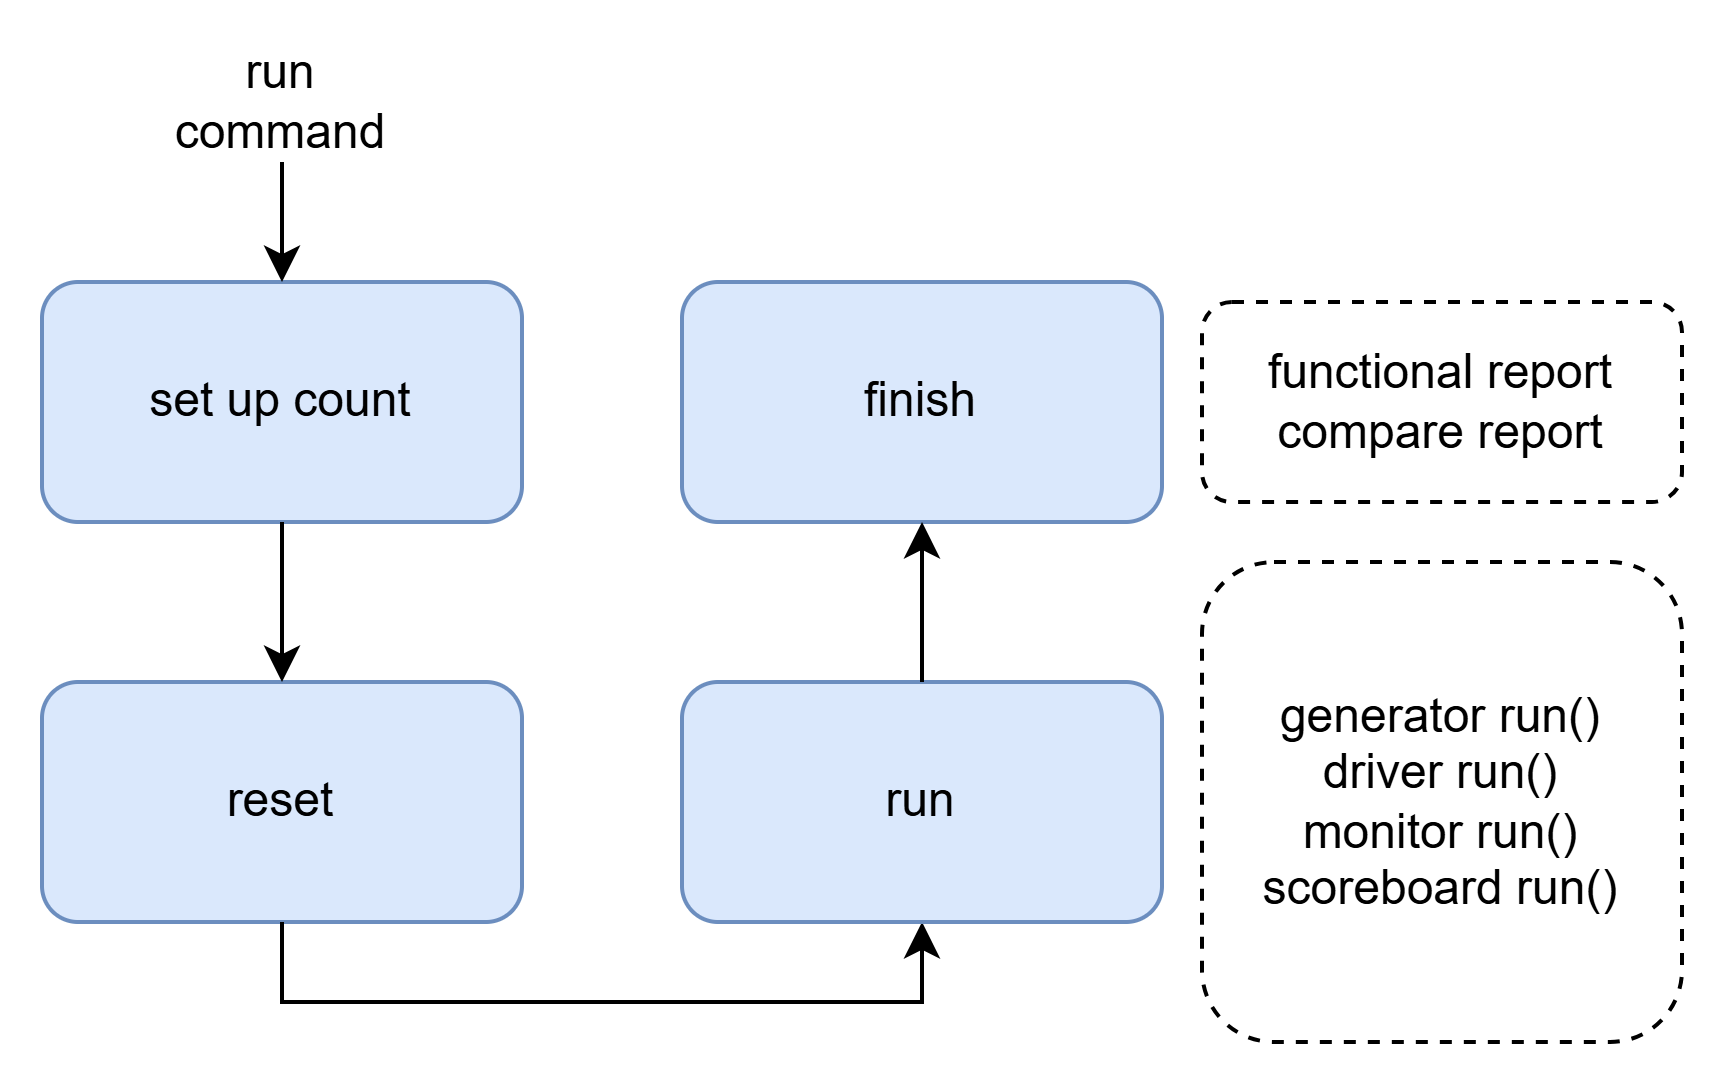
\includegraphics[width=1\linewidth]{figures/soc2.png}
	\caption{Luồng hoạt động của bộ kiểm thử}
	\label{fig:soc2}
\end{figure}

Hình \ref{fig:soc2} mô tả luồng hoạt động của bộ kiểm tra phân tầng. Bộ kiểm tra có thể tùy ý thay đổi số lượng test-bench kiểm tra dựa vào biến \textbf{count}. Sau khi đặt xong giá trị đếm, có thể bắt đầu kiểm tra hoạt động với hoạt động cài lại, sau đó các lớp con sẽ tiến hành chạy, sau khi đã hoàn thành đủ số lượng test-bench, tiến hành đưa ra 2 báo cáo bao gồm độ bao phủ chức năng và so sánh tỉ lệ chính xác với phiên bản phần mềm.
\begin{figure}[!ht]
	\centering
	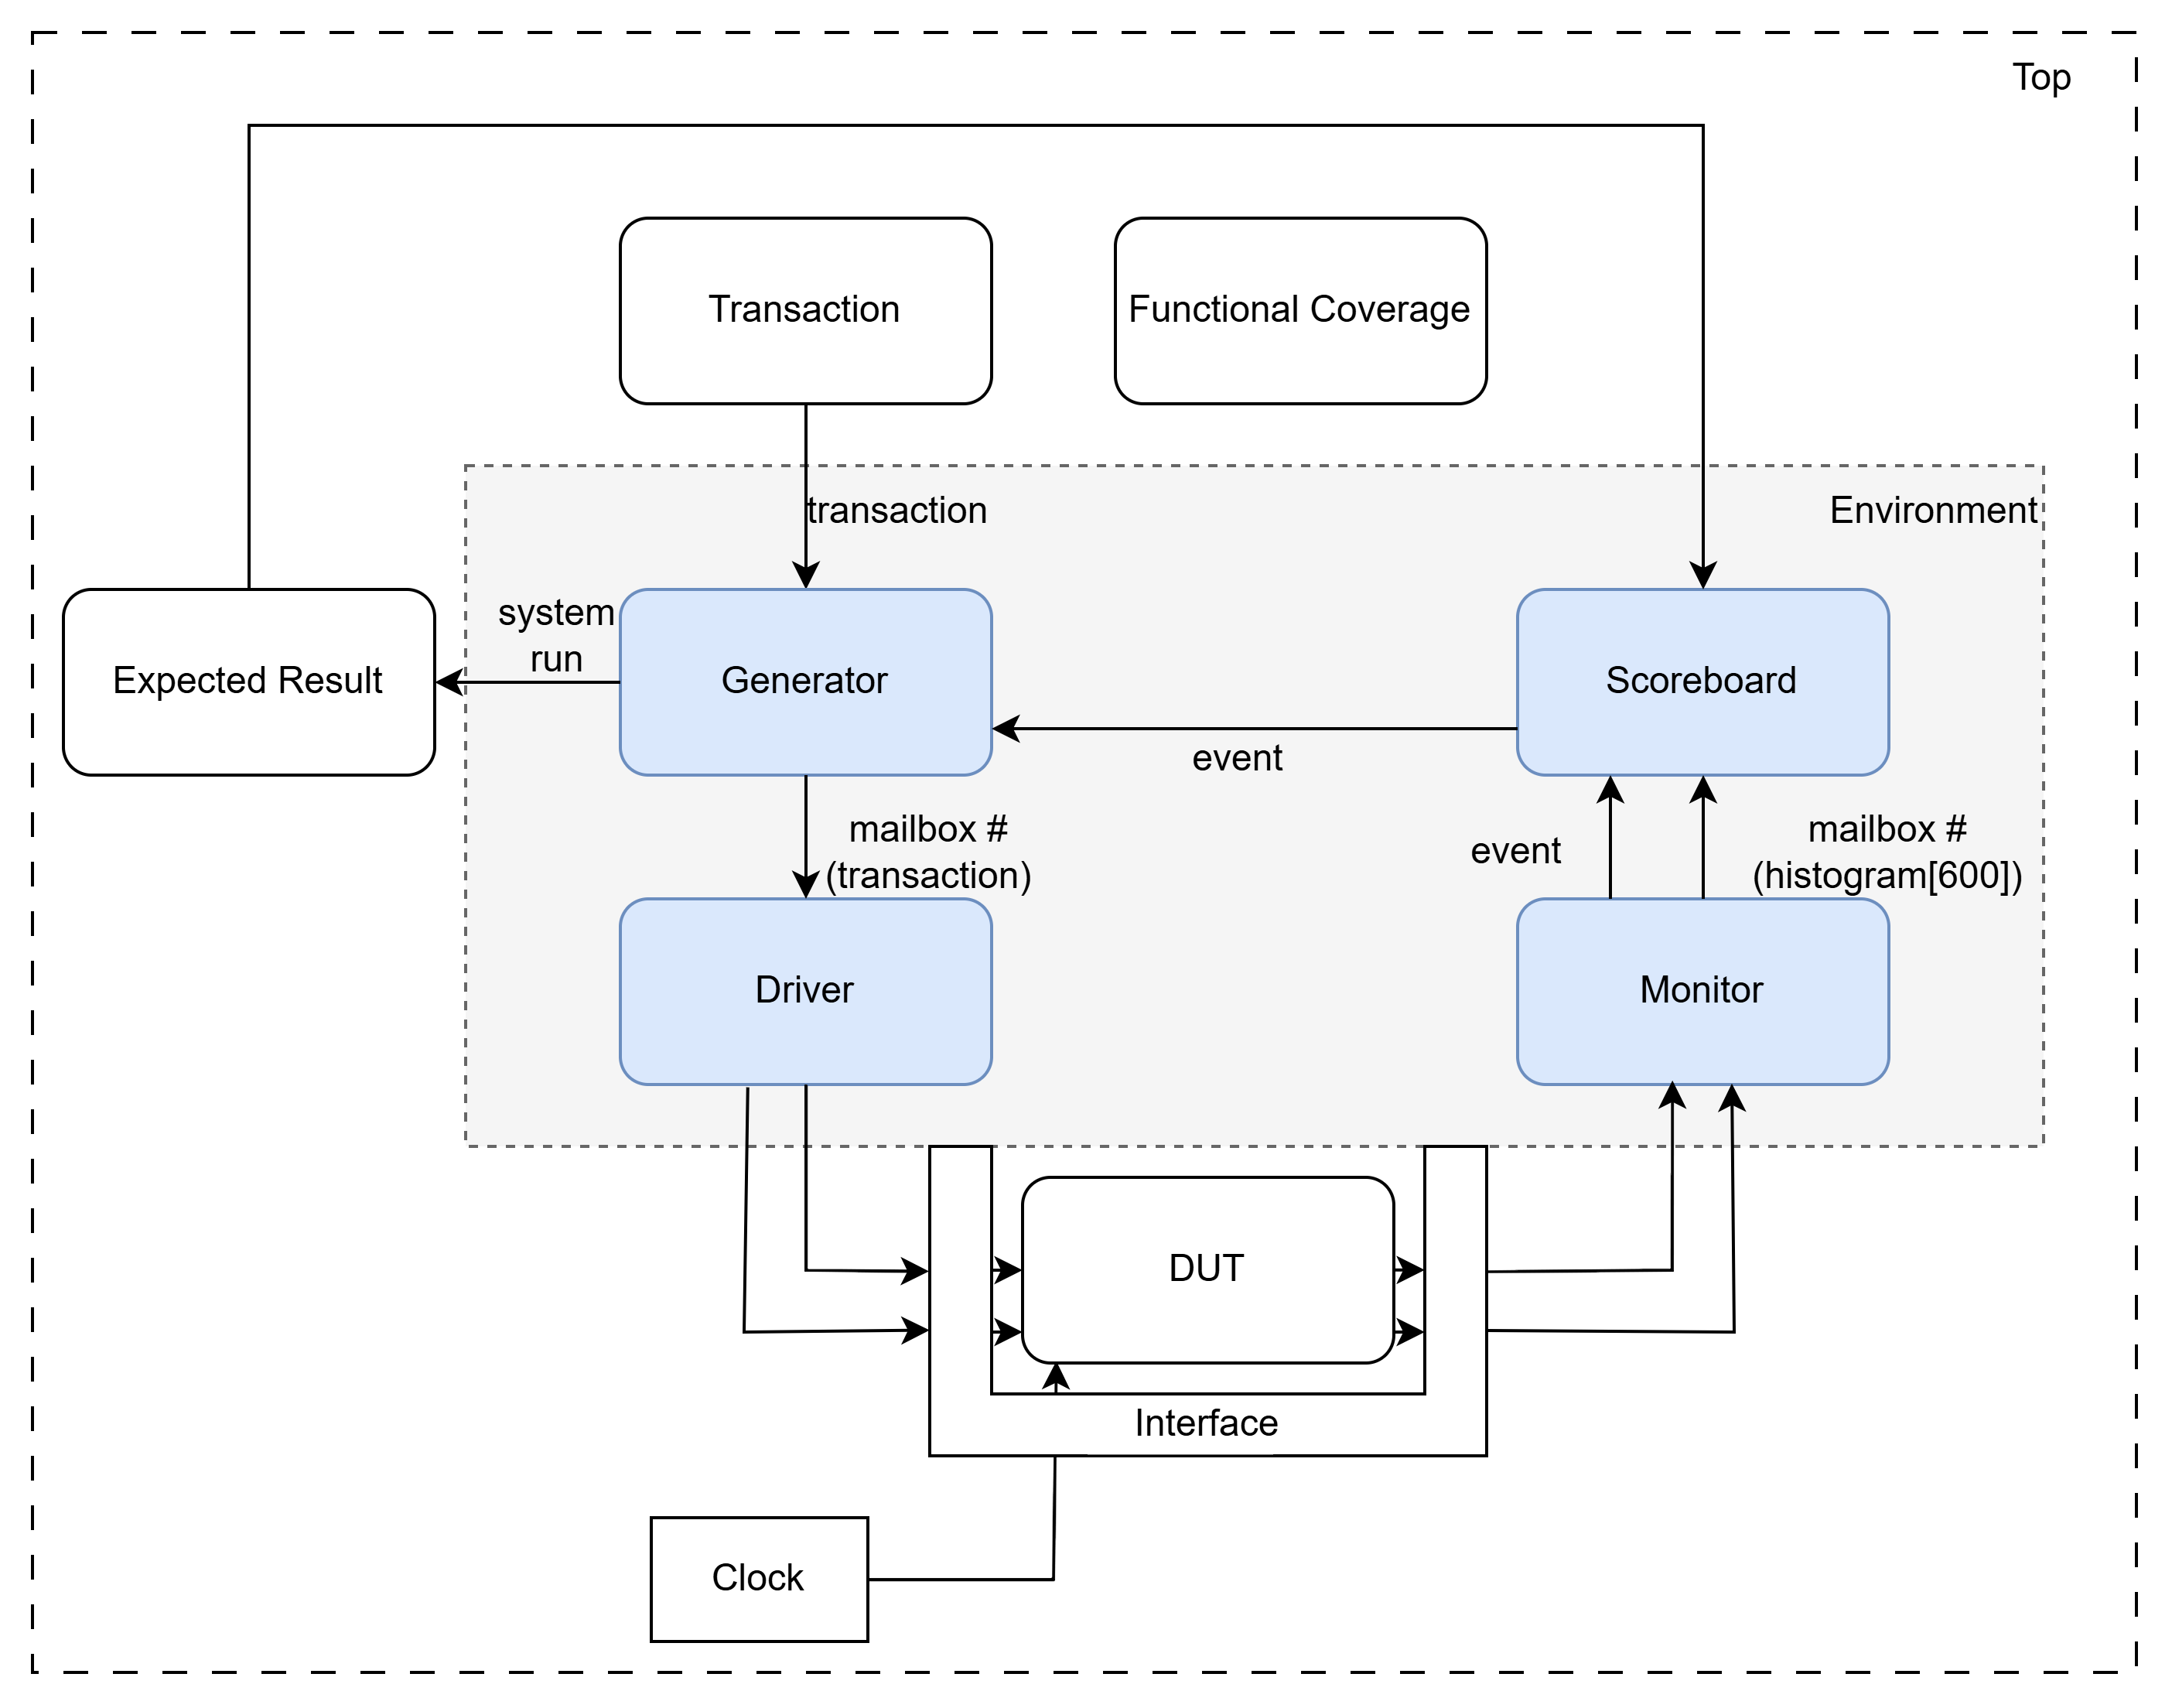
\includegraphics[width=\linewidth]{figures/myLayeredtb.png}
	\caption{Bộ kiểm tra phân tầng}
	\label{fig:myLayeredtb}
\end{figure}

Để đánh giá về độ bao phủ về mặt chức năng, kỹ sư cần đưa ra các điểm cần bao phủ. Đối với ngôn ngữ SystemVerilog, ngôn ngữ hỗ trợ các tính năng sau giúp đánh giá độ bao phủ:
\begin{itemize}
	\item Coverpoint - điểm bao phủ: là điểm mà sẽ thực hiện đánh giá bao phủ, thực chất điểm ở đây là các tín hiệu hoặc các biến
	\item Covergroup - nhóm bao phủ: là tập hợp các điểm bao phủ sẽ được lấy mẫu.
	\item Bins định nghĩa ra các trường hợp mà coverpoint sẽ cần xảy ra, nếu coverpoint xuất hiện giá trị được định nghĩa trong bins thì coi như là "hit" nếu không xuất hiện bất cứ lần nào thì là "miss".
	\item Cross: có thể gộp 2 hoặc nhiều coverpoint theo các tổ hợp có thể xảy ra với cross, ví dụ nếu định nghĩa coverpoint tín hiệu i\_valid, thì có thể cross i\_valid và dữ liệu để đánh giá xem trường hợp khi giá trị đầu vào là hợp lệ thì dữ liệu có hợp lệ hay không.
	\item Covergroup.get\_coverage(): sẽ đưa ra tỉ lệ hit trên tổng sổ các trường hợp có thể xảy ra của các coverpoint được định nghĩa trong covergroup đó.
\end{itemize}
%Sinh viên đã định nghĩa ra một vài trường hợp để đánh giá độ bao phủ về mặt chức năng được mô tả trong bảng \ref{tab:myFC}. Ngoài một vài các trường hợp được định nghĩa ở trong bảng thì một vài mô-đun sẽ có các trường hợp đánh giá riêng phù hợp cho mô-đun đó, ví dụ với mô-đun ZeroPadding thì sẽ cần đánh giá xem các trường hợp chuyển cửa sổ đệm có theo trình tự hay không.
%
%\begin{table}[H]
%	\centering
%	\renewcommand{\arraystretch}{1.3}
%		\caption{Các yếu tố để đánh giá độ bao phủ chức năng}
%	\begin{tabular}{|p{4cm} p{4cm} p{6cm}|}
%		\hline
%		\rowcolor{gray!30}
%		\textbf{Tên chức năng} & \textbf{Mô tả}  & Ví dụ  \\
%		\hline
%		Dữ liệu đầu vào và ra & Đánh giá dữ liệu vào có đủ hết trường hợp ứng với số bit của dữ liệu hay không & 8 bit sẽ chia thành các khoảng dữ liệu và kiểm tra xem dữ liệu có trong khoảng đấy không
%		\\ \hline
%		Đánh giá chuyển trạng thái & Đánh giá xem có chuyển hết các trạng thái đã định nghĩa hay không & Trạng thái đảm bảo chuyển từ \textit{READ->DONE->IDLE} trong 3 chu kỳ liên tiếp
%	
%		\\ \hline
%		Đánh giá điều kiện tín hiệu & Đánh giá xem tín hiệu có hoạt động đúng như mô tả trong đặc tả hay không & Tín hiệu o\_valid chuyển từ 1->0 đồng thời tín hiệu o\_finish chuyển từ 0->1 trong 2 chu kỳ liên tiếp và phải đồng thời
%		\\ \hline
%	\end{tabular}
%
%	\label{tab:myFC}
%\end{table}
%
%\textbf{Kết quả: } Bài kiểm thử với \textbf{1000} bài kiểm tra ngẫu nhiên cho độ bao phủ về mặt chức năng là \textbf{98\%}, trong khi đó độ khớp với kết quả mong muốn là \textbf{100\%}.




